\chapter{Visualize spectral distances}
\label{ch:visualize-spectral-distances}

\newthought{Let's consider a spectrum}, or any other data entry for that matter, as a point in a multidimensional space. We can define distance metrics between these points and visualize the distance values from one another or from a selected reference point or reference spectrum. By doing so, we can explore how similar our measurements are to a selected reference. We can do this on a series of spectra or even on hyperspectral maps!


\begin{figure}[h]
    \centering
	\vspace{0cm}
    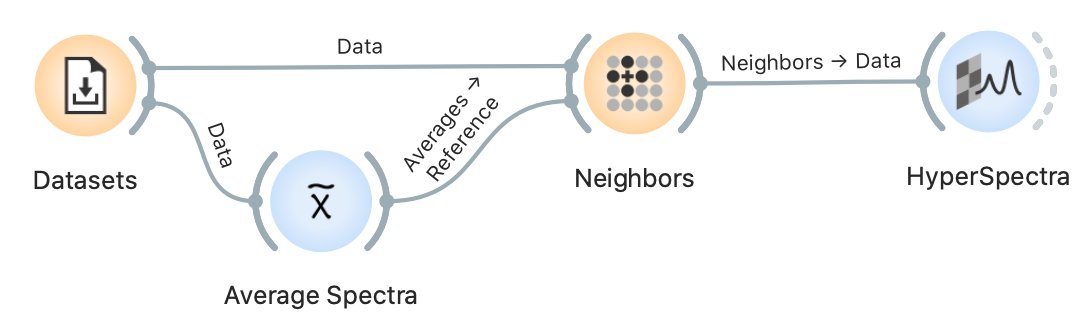
\includegraphics[width=\textwidth]{workflow.png}
    \caption{Load the \textit{'Liver cirrhosis - spectral image'} dataset from the \widget{Datasets} widget and calculate the \textit{Euclidean distances} from the average spectrum with the \widget{Neighbors} widget. Visualize them in \widget{Hyperspectra}.}
\end{figure}

\vspace{-0.5cm}

\noindent Can you reproduce the results below? Pay attention to the color scheme.

\begin{figure*}[h]
\centering
\vspace{-0.5cm}
\infinitewidthbox{
  \stackinset{r}{-0.5\linewidth}{t}{+0.1\linewidth}
  {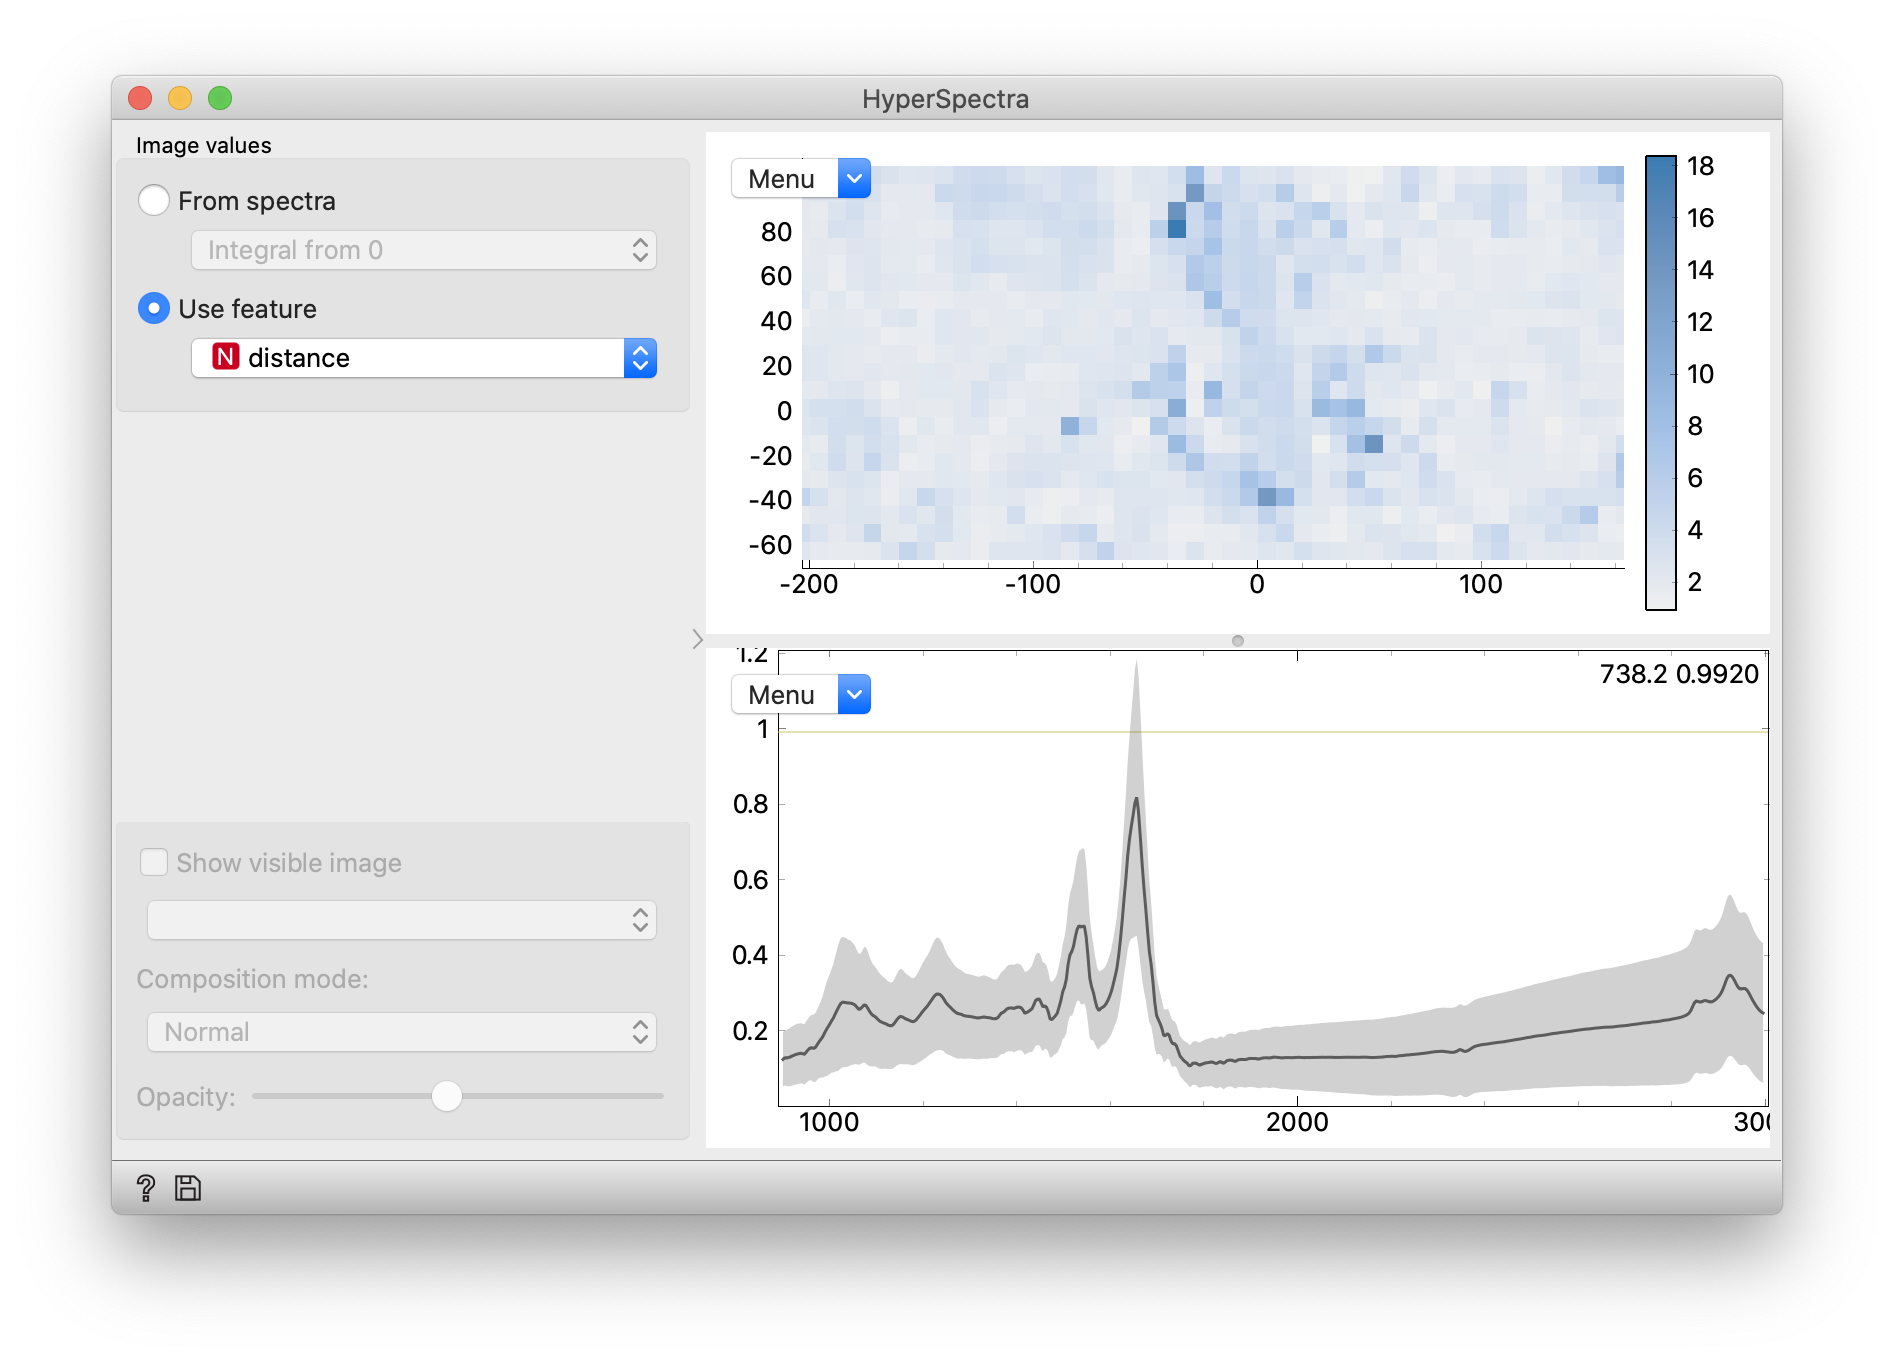
\includegraphics[scale=0.4]{ch-visualize_spectral_distances-fig3.png}}
  {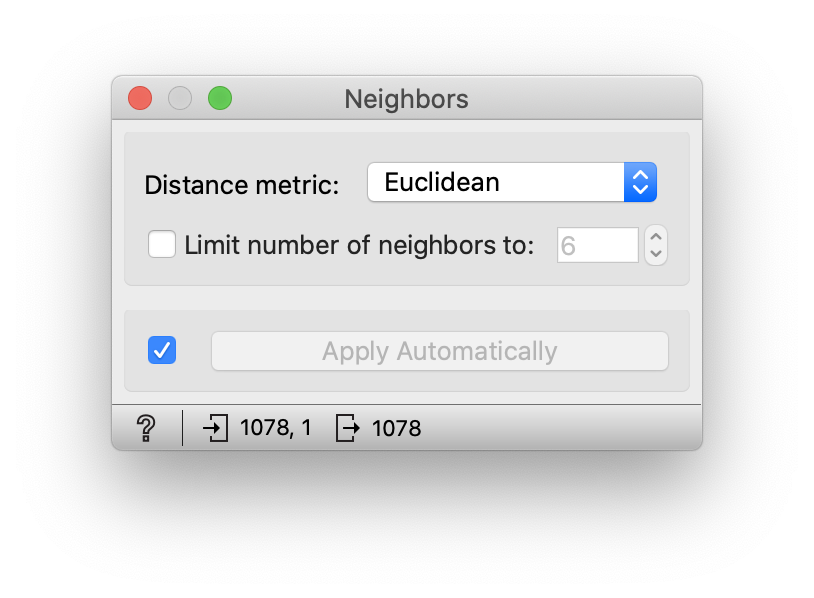
\includegraphics[scale=0.6]{ch-visualize_spectral_distances-fig2.png}}
  \hspace{8cm}
  }
%\caption{Try changing the parameters!}
\end{figure*}

\vspace{-0.5cm}

\noindent Explore different distance metrics, inspect distances in a \widget{Data Table} widget. Don't forget, you can select points on the top map and see the corresponding spectra on the bottom in \widget{Hyperspectra}.

\lecnotes{Possibility for discussion of the general mathematical properties of distance functions. See \url{https://en.wikipedia.org/wiki/Metric_(mathematics)}}